%First Latex document
\documentclass[pdftex]{article}
\usepackage{amsmath}
\usepackage[pdftex]{graphicx}
\begin{document}
\author{Prerana Pradhan}
\title{Undergraduate Research Report for Dr. Olson's Lab}
\maketitle
\section{Introduction}
During the Spring semester of 2008, the research conducted at Dr. Olson's lab consisted mainly of understanding and mastering the use of the 3DNA software. 
\subsection{The Importance of Nucleic Acids}
After the second part of the 20th century, the central dogma of biology consolidated and its main principle. 
\newline
\noindent
This is an example of how great Latex is for writing mathematical equations. 
\begin{gather}
\int \sin dx = - \cos x \\
\int \cos dx = \sin x  
\end{gather}
This is an example of putting a graph or figure in Latex.
\begin{figure}
\centering
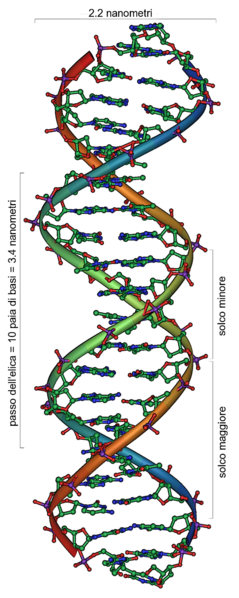
\includegraphics[scale=0.5]{dna.png}
\caption{Horrible Picture of DNA}
\end{figure}
\end{document}
